\documentclass{article}
\usepackage{graphicx} % Required for inserting images
\usepackage[Export]{adjustbox}

\title{Latihan Soal Matematika}

\begin{document}

\maketitle

\begin{enumerate}
    \item \begin{minipage}[t]{\linewidth}
          \raggedright
            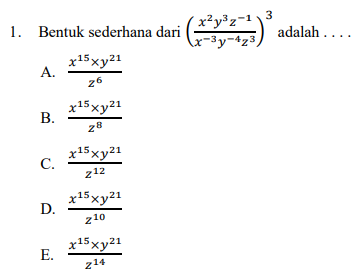
\includegraphics[valign=t]{1.png}\\
						Menggunakan sifat eksponen $(a^n)^m = a^{nm}$
						\[
							\left(\frac{x^{2}y^{3}z^{-1}}{x^{-3}y^{-4}z^{3}}\right)^3 = 
							\frac{x^{6}y^{9}z^{-3}}{x^{-9}y^{-12}z^{9}}
						\]
						Menggunakan sifat eksponen $a^{-n}=\frac{1}{a^n}$
						\[
							\frac{x^{6}y^{9}z^{-3}}{x^{-9}y^{-12}z^{9}} =
							\frac{x^{6}y^{9}x^{9}y^{12}}{z^{3}z^{9}}
						\]
						Menggunakan sifat eksponen $a^{n}\cdot a^{m}=a^{nm}$
						\[
							\frac{x^{6}y^{9}x^{9}y^{12}}{z^{3}z^{9}} = 
							\frac{x^{15} y^{21}}{z^{12}} \left(C\right)
						\]
					\end{minipage}
				\item \begin{minipage}[t]{\linewidth}
					\raggedright
						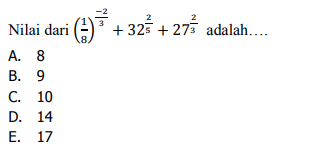
\includegraphics[valign=t]{2.png} \\
						Menggunakan sifat eksponen $a^{\frac{n}{m}}=\sqrt[n]{a^m}$
						\[
							\left(\frac{1}{8}\right)^{\frac{-2}{3}}+32^{\frac{2}{5}}+27^{\frac{2}{3}} = 
							\sqrt[3]{\left(\frac{1}{8}\right)^{-2}}+\sqrt[5]{32^{2}}+\sqrt[3]{27^{2}}
						\]
						Menggunakan sifat eksponen $\left(\frac{a}{b}\right)^{n}=\frac{a^{n}}{b^{n}}$
						\[
							\sqrt[3]{\left(\frac{1}{8}\right)^{-2}}+\sqrt[5]{32^{2}}+\sqrt[3]{27^{2}} =
							\sqrt[3]{\frac{1^{-2}}{8^{-2}}}+\sqrt[5]{32^{2}}+\sqrt[3]{27^{2}}	
						\]
						Menggunakan sifat eksponen $a^{-n}=\frac{1}{a^n}$
							\begin{align}
								\sqrt[3]{\frac{1^{-2}}{8^{-2}}}+\sqrt[5]{32^{2}}+\sqrt[3]{27^{2}} &= 
								\sqrt[3]{\frac{\frac{1}{1^{2}}}{\frac{1}{8^{2}}}}+\sqrt[5]{32^{2}}+\sqrt[3]{27^{2}}\\
								&=90141 \\
							\end{align}
						\end{minipage}
    
\end{enumerate}

\end{document}
